 \chapter{Materials and Methods}

 \section{Motion Segmentation }
As reported in D9, we developed a novel motion segmentation algorithm utilizing neuromorphic vision sensor. The algorithm was characterized by experiments in controlled environments. The paper has been submitted to Frontiers in Neuroscience. The next step was to integrate the algorithm with a virtual reality platform, allowing a controller to remotely visualize the environment and interact with the robot.
\begin{figure}[h!]
	\begin{center}
		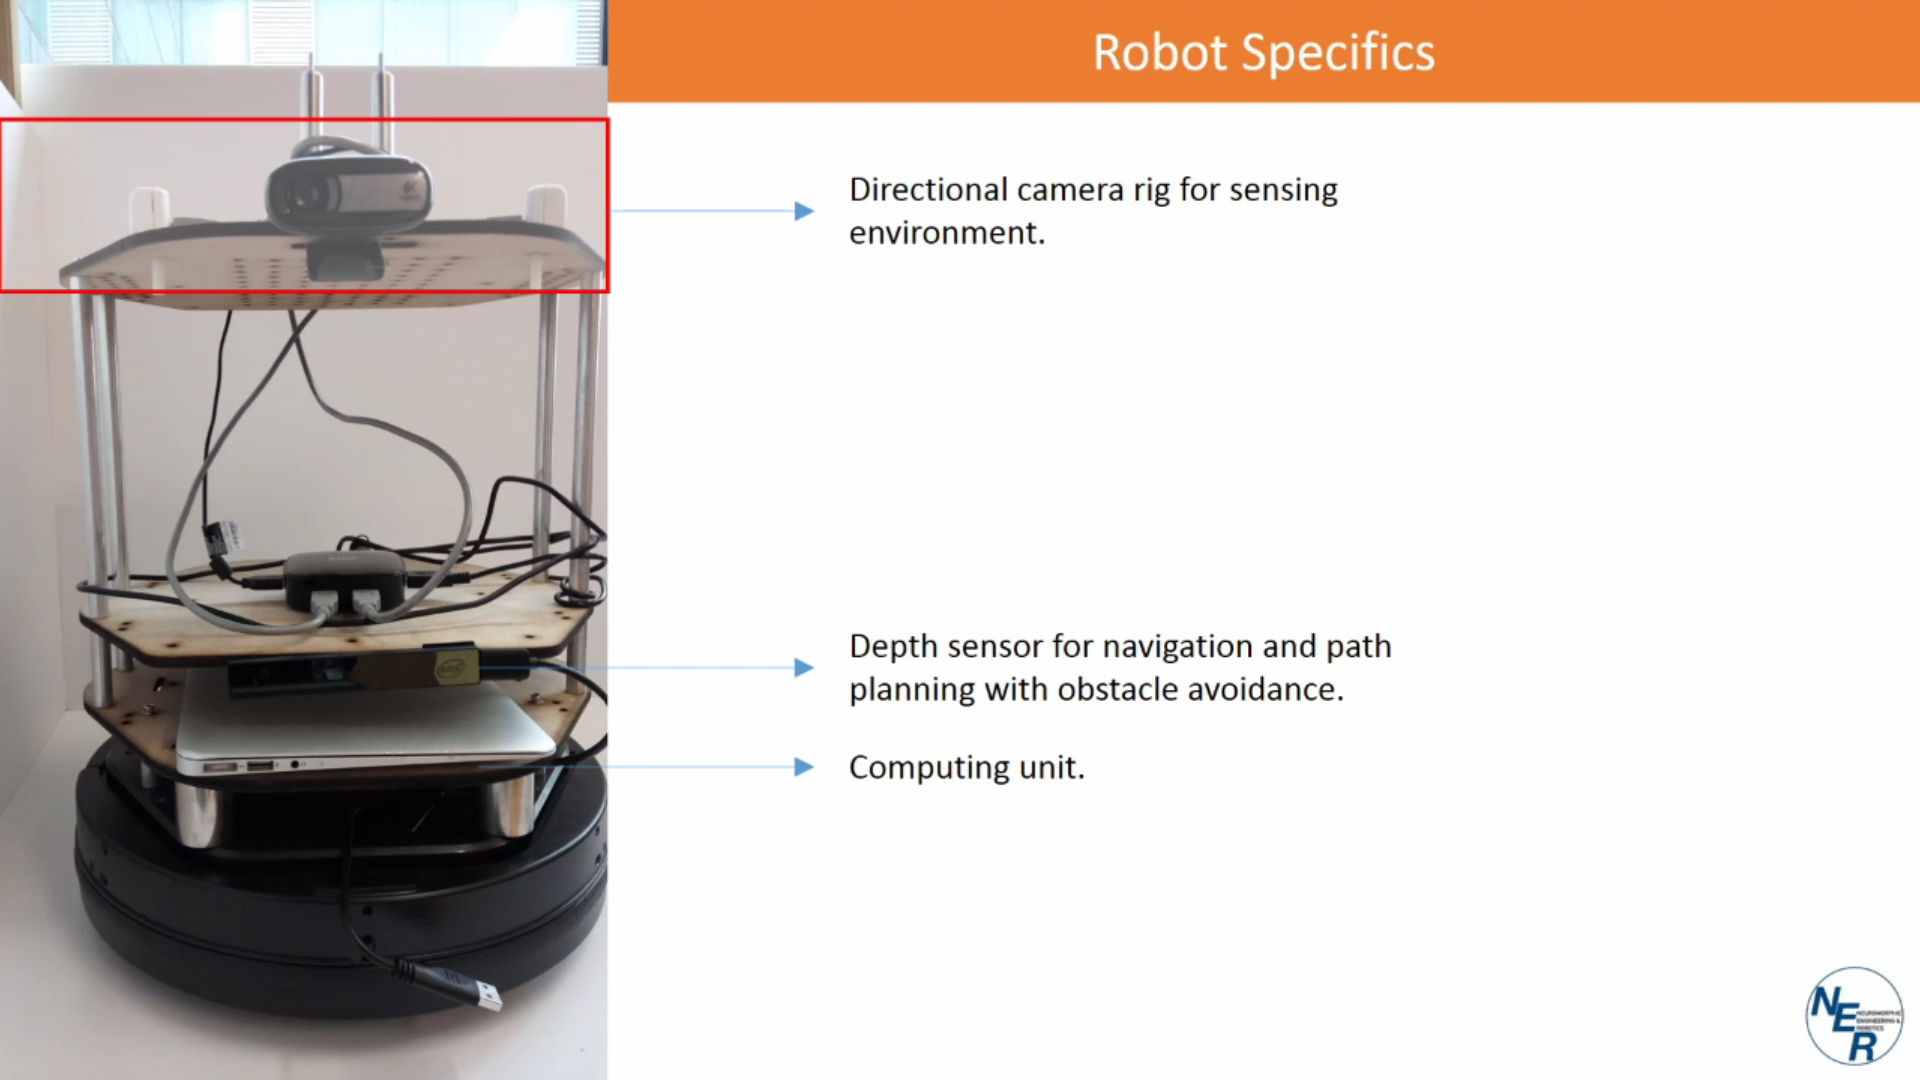
\includegraphics[width=0.90\textwidth]{figures/motion-seg/setup}% This is a *.jpg file
	\end{center}
	\textbf{\refstepcounter{figure}\label{fig:turtle_setup} Figure \arabic{figure}. Sensor integration in the robotic platform for experiments.}. { The robot is ROS-enabled and allows development of algorithms within the ROS ecosystem. }
\end{figure}

In this report, we emphasize on the development of (1) the robotic platform for integrating various sensors for navigation and motion segmentation and (2) wireless data transfer and rendition in a virtual reality platform. As shown in Figure~\ref{fig:turtle_setup}, we use the turtlebot robotic platform to integrate the sensors and algorithms. The robot comprises three USB cameras with their field of views (FoV) aligned such that they form a continuous scene when rendered consecutively. The robot is equipped with a RGBD sensor, Intel's RealSense R200, allowing the robot to make a map of its environment and perform path planning. A central computing unit is responsible for executing the algorithms for path planning, obstacle avoidance, motion segmentation and wireless environment image transfer. 

Figure~\ref{fig:VR_setup} shows the corresponding data as received by the virtual reality platform. The current implementation uses image data encoded as a motion-JPEG (mjpg) video stream at $20fps$, rendered by a viewer such as a web browser. The robot is located in a remote location and implements the algorithms for navigation, path planning and obstacle avoidance.
\begin{figure}[h!]
	\begin{center}
		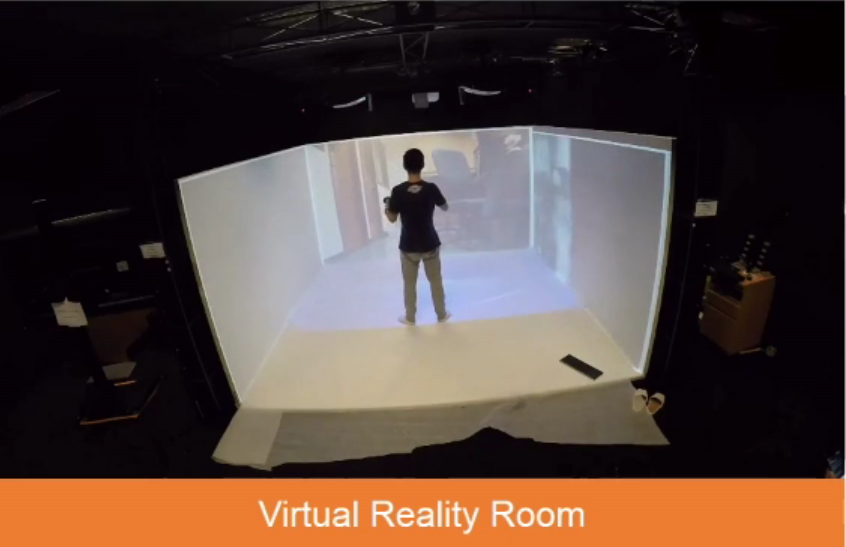
\includegraphics[width=0.90\textwidth]{figures/motion-seg/VR-Robot}% This is a *.jpg file
	\end{center}
	\textbf{\refstepcounter{figure}\label{fig:VR_setup} Figure \arabic{figure}. Rendition of data from the robot.} { Data from the three directional cameras installed on the robot is displayed in the virtual reality platform. }
\end{figure}

Figure~\ref{fig:robot-env}(A) shows the 2D map that is calculated and stored locally on the robot's computing unit for navigation and obstacle avoidance. The arrow indicates the location of the robot in the map with the corresponding physical location as shown in Figure~\ref{fig:robot-env}(B). A gesture tracking algorithm was developed that manipulates robot's motion parameters in real-time.
\begin{figure}[h!]
	\begin{center}
		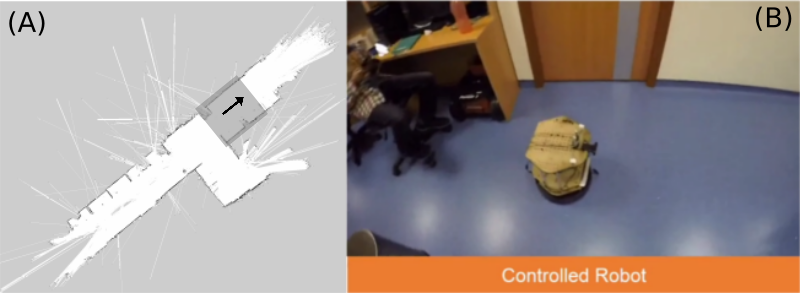
\includegraphics[width=0.95\textwidth]{figures/motion-seg/robot-env}% This is a *.jpg file
	\end{center}
	\textbf{\refstepcounter{figure}\label{fig:robot-env} Figure \arabic{figure}. Robot's map and physical location.} { (A) A 2D map created using the RGBD sensor is shown. (B) The corresponding physical location of the robot is shown. }
\end{figure}

\section{Vibro-Tactile Haptic Glove}
The second generation of vibro-tactile haptic gloves was developed. These gloves have the capability of rendering spatial touch information with amplitude modulation. The high-density gloves have 18 vibratory eccentric rotating mass actuators. The actuator locations were selected to deliver haptic feedback at the most used and sensitive areas on the palm-side of the hand during exploratory procedures. The actuators are held in place by a flexible PCB, made from polyimide, to closely represent the topography of the hand, minimize wiring complexities, prevent displacements after prolonged usage and give a more natural skin-like feel.
The control box is placed at the wrist location. The vibration
intensity and their activation is controlled wirelessly through a
graphical user interface (GUI) that is designed to send custom
stimulation patterns. The GUI enables single and multiple actuator
activation with amplitude modulation for intensity control. In near-field operation the latency is low permitting real-time feedback. The control box consists of two pulse width modulation (PWM) drivers and one Arduino microcontroller. The computer transmitting an encoded stimulation signal received by the control box initiates the communication pathway. This signal is sent to a microcontroller for actuation. In addition, the control box contains a power source for the system. A prototype of the second generation haptic glove is show in Figure 1. 

As reported in D9 report, we developed the second generation
vibro-tactile gloves with flexible PCB to reduce wiring. However due
to the stiffness of the PCB and the dissipation of vibro-tactile
stimuli on the palm region experienced by the user, we developed third
generation of vibrotactile glove. In this version, we use wires to
fasten the actuators and give the user a more natural feel.

In the third-generation, eighteen actuators are placed at sensitive
locations of human’s hand. This generation of haptic glove is flexible and light weight. 


\section{VR Simulation}
We aim at rendering complex virtual objects as shown in Figure 2, to
the user by mapping their shapes to the vibratory stimuli on the
haptic glove.

A VR environment is built inside the CAVE with 4 projectors using
Unity development platform. We have developed a pick and place VR
simulation as shown in Figure 3. We are evaluating strategies for the
rendition of 3-dimensional geometric shapes to the user with the
vibro-tactile glove.

An ART D-track system as shown in Figure 4, is used to track the position and the movement of a user accurately in the VR environment. The ART-DTracking(Advanced Realtime Tracking) system, which is used for interaction in this case, will be used for providing gesture data. Simple clustering algorithms are used to locate the human hand and body. The position data is then translated and recorded into position data in the VR system for further usage. 


This tracking system will also be used by a tele-operator to interact
with a virtual avatar of the robot deployed in a remote
location. Depth sensors like RealSense or Kinect are used to render
the scene around robot in the VR environment.

